\section{Teilaufgabe 1}
\begin{aufgabe}
    Zeichnen Sie den Wirkungsplan der obigen Differentialgleichung und 
    programmieren Sie diesen Wirkungsplan im Simulink. Führen Sie ein paar 
    Simulationen durch und prüfen Sie die Plausibilität der Ergebnisse. Sie 
    sollten auch unterschiedliche Anfangsbedingungen für die Drehzahl testen.
\end{aufgabe}
\[ \dot{\omega}(t) 
    = -\frac{1}{J} \cdot \left(\alpha + \frac{K^2}{R}\right) \cdot \omega(t) 
    + \frac{K}{J \cdot R} \cdot u(t) - \frac{1}{J} \cdot \Gamma_l(t) \]
\begin{figure}[h!]
    \centering
    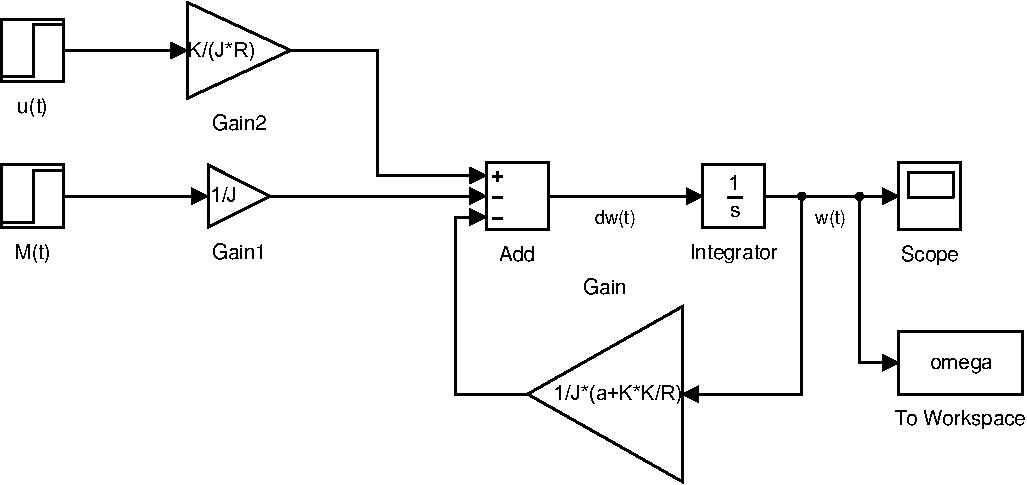
\includegraphics[width=0.6\textwidth]{01/wirkungsplan.pdf}
    \caption{Wirkungsplan DGL}
    \label{fig:01}
\end{figure}
\begin{figure}[h!]
    \centering
    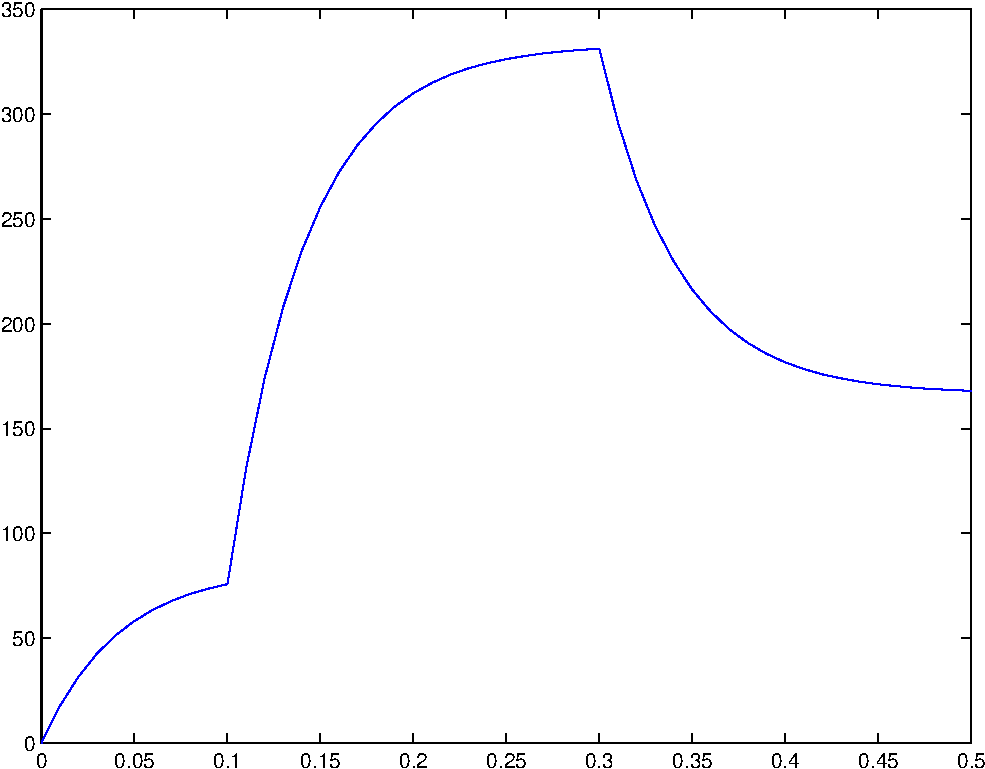
\includegraphics[width=0.6\textwidth]{01/wirkungsplan_plot.pdf}
    \caption{Simulationsergebnis}
    \label{fig:01plot}
\end{figure}
\lstinputlisting{01/wirkungsplan.m}
